\documentclass[12pt]{article}
%% If uncommented, will use the minted package. This requires python and latex to compile with --shell-escape.
%% Otherwise, just use listings
% \newcommand*{\UsePackageMinted}{}

\usepackage[margin=1in, left=0.6in, right=0.6in]{geometry}
\usepackage{fancyhdr} % header
\usepackage{hyperref} % links
\usepackage{amsmath,amsthm,amssymb}	%math stuff
\usepackage{setspace} % increase line spacing
\usepackage[table]{xcolor} % align environment
\usepackage{changepage} % for the adjustwidth environment
\usepackage{relsize} % Scaling the font
\usepackage{algorithm} % for algorithms
\usepackage{caption} % captioning the algorithm
\usepackage[export]{adjustbox}% http://ctan.org/pkg/adjustbox
\usepackage{graphicx} \graphicspath{ {./images/} } % images
\usepackage[noend]{algpseudocode} % pseudo code
\usepackage[T1]{fontenc} % for {} in \texttt{}

%% with the minted package, have to compile manually with `pdflatex -shell-escape cscc73-a1.tex`, or make termporary
%% ~/.latexmkrc
%% with the following contents
% $latex = 'latex  %O  --shell-escape %S';
% $pdflatex = 'pdflatex  %O  --shell-escape %S';
\ifdefined\UsePackageMinted
	\usepackage{minted} % original, but requires python
\else
	% Python
	% Default fixed font does not support bold face
	\DeclareFixedFont{\ttb}{T1}{txtt}{bx}{n}{12} % for bold
	\DeclareFixedFont{\ttm}{T1}{txtt}{m}{n}{12}  % for normal

	% Custom colors
	\usepackage{color}
	\definecolor{deepblue}{rgb}{0,0,0.5}
	\definecolor{deepred}{rgb}{0.6,0,0}
	\definecolor{deepgreen}{rgb}{0,0.5,0}

	\usepackage{listings}
	% Python style for highlighting
	\newcommand\pythonstyle{\lstset{
	language=Python,
	basicstyle=\ttm,
	morekeywords={self},              % Add keywords here
	keywordstyle=\ttb\color{deepblue},
	emph={MyClass,__init__},          % Custom highlighting
	emphstyle=\ttb\color{deepred},    % Custom highlighting style
	stringstyle=\color{deepgreen},
	frame=tb,                         % Any extra options here
	showstringspaces=false,
	morestring=[s]{"""}{"""}
	}}

	% Python environment
	\lstnewenvironment{python}[1][]
	{
	\pythonstyle
	\lstset{#1}
	}
	{}
\fi

\setlength{\parindent}{0pt}
\everymath{\displaystyle}

\pagestyle{fancy}
\fancyhead[LO,L]{CSCC73 A1}
\fancyhead[CO,C]{Stephen Guo, Ezzeldin Ismail}
\fancyhead[RO,R]{1006313231, 1005798861}
\fancyfoot[LO,L]{}
\fancyfoot[CO,C]{\thepage}
\fancyfoot[RO,R]{}

\begin{document}
%----------------------------------------------------------------------------------
%                              Table of Contents
%----------------------------------------------------------------------------------
\begin{center}
	\hypertarget{toc}{\LARGE \underline{\textbf{Table of Contents}}}\\
\end{center}

\hyperlink{1}{\textbf{Question 1:}}
\vspace{1mm}
\hrule
\vspace{1mm} \leavevmode \\

\hyperlink{2}{\textbf{Question 2:}}
\vspace{1mm}
\hrule
\vspace{1mm} \leavevmode \\

\newpage

%----------------------------------------------------------------------------------
%                                   Questions
%----------------------------------------------------------------------------------
\setstretch{1.2}
%----------------------------------------------------------------------------------
% !                                     1
%----------------------------------------------------------------------------------
\hyperlink{toc}{\hypertarget{1}{\LARGE \underline{\textbf{Question 1.}}}}\\
\begin{algorithm}
	\caption*{\textbf{Algorithm}\\Min\_Stage2 \big(\texttt{jobs}: array of tuples $(j_i,\ s_i)$\big)}\label{alg:cap}
	\begin{algorithmic}[1]
		\State sort \texttt{jobs} by $s_i$ decreasing
		\State return \texttt{jobs}
	\end{algorithmic}
\end{algorithm}

As we can see, \texttt{Min\_Stage2()} is a greedy algorith with a choice of longest stage 2.
\texttt{Min\_Stage2()} gives a feasible output since we just return a reordered list of the original list of jobs.\\

\textbf{Claim}: Swapping an earlier job with a later job that has a longer stage 2 will not make the end time worse.\\
\textbf{Proof}:
\begin{adjustwidth}{10mm}{}
	Let $f_i,\ s_i$ be the earlier job with a shorter stage 2\\
	Let $f_j,\ s_j$ be the later job with a longer stage 2\\
	$\Longrightarrow s_j \geq s_i$\\
	Let end time be the time it takes for both stages of the job to finish\\

	Before swapping, we have\\
	{
	\setstretch{1.5}
	$
		\begin{array}{r@{}>{\displaystyle}ll}
			\text{end time}(s_i)   & {}=f_i + s_i                                        &                                            \\
			\text{end time}(s_j)   & {}=f_i  + f_j + s_j                                 &                                            \\
			\text{latest end time} & {}=\text{max}\big(f_i + s_i,\ f_i  + f_j + s_j\big) &                                            \\
			                       & {}= f_i  + f_j + s_j                                & \hspace*{5mm}[\text{since $s_j \geq s_i$}] \\
		\end{array}
	$
	}\\[5mm]

	After swapping, we have\\
	{
	\setstretch{1.5}
	$
		\begin{array}{r@{}>{\displaystyle}ll}
			\text{end time}(s_i)^\prime   & {}=f_j  + f_i + s_i                                 & \\
			\text{end time}(s_j)^\prime   & {}=f_j + s_j                                        & \\
			\text{latest end time}^\prime & {}=\text{max}\big(f_j + s_j,\ f_j  + f_i + s_i\big) & \\
		\end{array}
	$
	}\\[5mm]

	in all cases, latest end time $\geq$ latest end time$^\prime\hspace*{\fill}\blacksquare$
\end{adjustwidth}

\newpage
\textbf{Theorem}: Greedy schedule $S$ given by \texttt{Min\_Stage2()} is optimal\\
\textbf{Proof} (Exchange argument):
\begin{adjustwidth}{10mm}{}
	Let $O$ be an optimal ordering of jobs ${O\text{-job}}_i$\\
	Let $S$ be the ordering of jobs ${S\text{-job}}_i$ given by \texttt{Min\_Stage2()}\\
	{
	\setstretch{1.5}
	$
		\begin{array}{r@{}>{\displaystyle}l}
			\text{Suppose\hspace*{5mm}} {O\text{-job}}_1 & {}= {S\text{-job}}_1       \\
			{O\text{-job}}_2                             & {}= {S\text{-job}}_2       \\[-2mm]
			                                             & \hspace*{2.5mm} \vdots     \\[-3mm]
			{O\text{-job}}_{i-2}                         & {}= {S\text{-job}}_{i-2}   \\
			{O\text{-job}}_{i-1}                         & {}= {S\text{-job}}_{i-1}   \\[4mm]
			\text{but }{O\text{-job}}_{i}                & {}\not= {S\text{-job}}_{i} \\
		\end{array}
	$
	}\\

	\textbf{WTS}: We can change order of $O$ to make it more similar to $S$ and the end time will not be any worse\\

	Let the remaining different jobs be\\
	$O\text{-Remaining} = [{O\text{-job}}_{i},\ {O\text{-job}}_{i+1},\ \cdots\ ,\ {O\text{-job}}_{n}]$ for $O$, and \\
	$S\text{-Remaining} = [{S\text{-job}}_{i},\ {S\text{-job}}_{i+1},\ \cdots\ ,\ {S\text{-job}}_{n}]$ for $S$\\

	since ${S\text{-job}}_{i} \not = {O\text{-job}}_{i}$, and $S\text{-Remaining}$ are sorted decreasing by longest stage 2's,
	then we can swap ${O\text{-job}}_{i}$ with a job that has the longest stage 2. Namely, continously swap ${O\text{-job}}_{i}$ with the left job until it reaches the
	${S\text{-job}}_{i}$'s position in $S$\\

	We can repeat this until $O\text{-Remaining} = S\text{-Remaining}$\\
	$\Longrightarrow O$ becomes more similar to $S$.\\
	and by the claim above, the end time does not get worse. $\hspace*{\fill}\blacksquare$
\end{adjustwidth}~\\
\texttt{Min\_Stage2()}'s complexity is $\mathcal{O}(n \log n)$ since it's simply sorting
\newpage
%----------------------------------------------------------------------------------
% !                                     2
%----------------------------------------------------------------------------------
\hyperlink{toc}{\hypertarget{2}{\LARGE \underline{\textbf{Question 2.}}}}\\\\
Our objective is to minimize the number of edges to add to get zero skew.\\

To attain this it's important to notice that increasing the length of an edge closer to the root increases the edge of $2^d$ leaves
where $d$ is the depth of that node at the end of the edge. Therefore, we should attempt to increase edge lengths greedily starting from the root,
ensuring that the increase does not push one of the distances above the current maximum. This is because if we increase the maximum distance,
we would at least not change the skew, or even risk the chance of increasing it.\\

This algorithm is done with an augmented binary tree,
where each node stores the distance between it and the root and the maximum distance from the root to any of its subtree leaves: i.e.
\begin{center}
	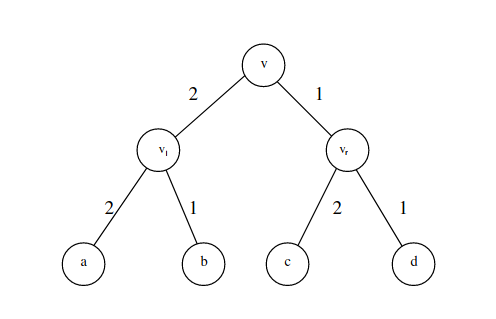
\includegraphics[scale=2,valign=m]{cscc73-a1-a2-diagram1.png}
	$\Longrightarrow\hspace*{5mm}$
	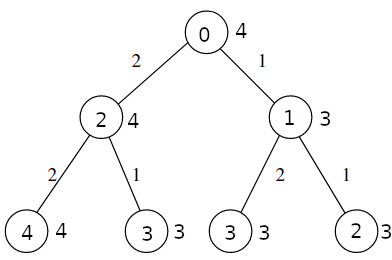
\includegraphics[width=66mm,valign=m]{cscc73-a1-a2-diagram2.jpeg}
\end{center}
% original
\ifdefined\UsePackageMinted
	\textbf{Algorithm}:
	\begin{minted}{python}
"""
BTree has shape
{
 left:
    {
     length: int
     node: BTree
    }
 right:
    {
     length: int
     node: BTree
    }
}
AugmentedBTree has shape
{
 max: int
 distance: int
 left: AugmentedBTree
 right:AugmentedBTree
}
"""
def zero_skew(orig: BTree):
    def augment(root, distance):
        if (root.left == None and root.right == None):
            return Node(dist=distance, max=distance, left=None, right=None)
        left = augment(root.left.node, root.left.length + distance)
        right = augment(root.right.node, root.right.length + distance)
        return Node(dist=distance, max=max(left.max, right.max), left=left, right=right)

    AugmentedTree = augment(orig, 0)
    max_d = AugmentedTree.max

    def increase_length(root, inc):
        root.dist += inc
        root.max += inc
        if (root.left == None and root.right == None):
            root.dist = max_d
        elif root.max == max_d:
            root.left = increase_length(root.left, inc)
            root.right = increase_length(root.right, inc)
        else:
            i = max_d - root.max
            root.dist += i
            root.right = increase_length(root.right, i)
            root.left = increase_length(root.left, i)
        return root

    return increase_length(AugmentedTree, 0)
\end{minted}
\else
	\newpage
	\textbf{Algorithm}:
	{
	\relscale{.5}
	\begin{python}
"""
BTree has shape
{
  left: {
	  length: int
	  node: BTree
	}
  right: {
    length: int
    node: BTree
  }
}

AugmentedBTree has shape
{
  max: int
  distance: int
  left:  AugmentedBTree
  right: AugmentedBTree
}
"""
def zero_skew(orig: BTree):
    def augment(root, distance):
        if (root.left == None and root.right == None):
            return Node (
                dist=distance,
                max=distance,
                left=None,
                right=None
            )
        left = augment(root.left.node, root.left.length + distance)
        right = augment(root.right.node, root.right.length + distance)
        return Node(
            dist=distance,
            max=max(left.max,right.max),
            left=left,
            right=right
        )

    AugmentedTree = augment(orig, 0)
    max_d = AugmentedTree.max

    def increase_length(root, inc):
        root.dist += inc
        root.max += inc
        if (root.left == None and root.right == None):
             root.dist = max_d
        elif root.max == max_d:
            root.left = increase_length(root.left, inc)
            root.right = increase_length(root.right, inc)
        else:
            i = max_d - root.max
            root.dist += i
            root.right = increase_length(root.right, i)
            root.left = increase_length(root.left, i)
        return root

    return increase_length(AugmentedTree, 0)
\end{python}
	}
\fi
\newpage

\texttt{zero\_skew()} gives a feasible solution since the algorithm copies the tree with more info, then starts increasing the length.\\
The greedy choice is the first node to increase the length.\\
In terms of complexity, it is clear that all operations done in \texttt{zero\_skew()} are inorder traversals of the input tree and therefore the total complexity is $O(n)$.\\

Proof of correctness (Exchange argument):
\begin{adjustwidth}{10mm}{}
	Since the operations of this algorithm are done in an inorder traversal, I will argue without loss of generality about one path.\\

	Let $A$ be the solution given by the greedy algorithm and $A^{opt}$ be an optimal solution.\\
	Let $b$ be a path between the root and a leaf node in A, and $b^{opt}$ be the path in $A^{opt}$\\
	Let $n$ be the first node differing between $b$ and $b^{opt}$.\\

	It cannot be that the node is larger in $b^{opt}$ than $b$ because then the greedy algorithm did not increase that node because increasing it would cause the the maximum distance to increase,
	which cannot happen in an optimal solution. So $n$ is larger in $b$ than $b^{opt}$.
	But this means that both left and right paths of the node in $b^{opt}$ have an increase,
	as some nodes in both paths are below the maximum distance (which we know because the node was increased in $b$).
	Therefore, we can remove 1 from each of the subsequent nodes in the left and right branches and increase $n$ in $b^{opt}$.
	But then we just reduced the amount of additions without going over the maximum distance in $b^{opt}$ which goes against the assumption that $b^{opt}$ is an optimal solution.
	So there cannot be an optimal solution that differs from the greedy solution.\\

	$\therefore$ \texttt{zero\_skew()} gives optimal solutions.
\end{adjustwidth}~\\[-9mm]
\end{document}
